% Created by tikzDevice version 0.8.1 on 2015-05-31 14:38:55
% !TEX encoding = UTF-8 Unicode
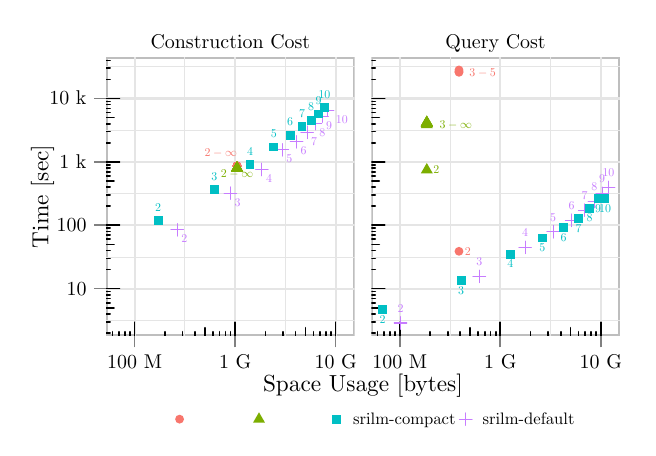
\begin{tikzpicture}[x=1pt,y=1pt]
\definecolor{fillColor}{RGB}{255,255,255}
\path[use as bounding box,fill=fillColor,fill opacity=0.00] (0,0) rectangle (216.81,144.54);
\begin{scope}
\path[clip] (  0.00,  0.00) rectangle (216.81,144.54);
\definecolor{fillColor}{RGB}{255,255,255}

\path[fill=fillColor] (  0.00,  0.00) rectangle (216.81,144.54);
\end{scope}
\begin{scope}
\path[clip] ( 28.36,133.83) rectangle (118.15,144.54);

\path[] ( 28.36,133.83) rectangle (118.15,144.54);
\definecolor{drawColor}{RGB}{0,0,0}

\node[text=drawColor,anchor=base,inner sep=0pt, outer sep=0pt, scale=  0.72] at ( 73.25,136.84) {Construction Cost};
\end{scope}
\begin{scope}
\path[clip] (124.17,133.83) rectangle (213.96,144.54);

\path[] (124.17,133.83) rectangle (213.96,144.54);
\definecolor{drawColor}{RGB}{0,0,0}

\node[text=drawColor,anchor=base,inner sep=0pt, outer sep=0pt, scale=  0.72] at (169.07,136.84) {Query Cost};
\end{scope}
\begin{scope}
\path[clip] ( 28.36, 33.25) rectangle (118.15,133.83);
\definecolor{drawColor}{RGB}{190,190,190}

\path[draw=drawColor,line width= 1.5pt,line join=round,line cap=round] ( 28.36, 33.25) rectangle (118.15,133.83);
\definecolor{drawColor}{gray}{0.90}

\path[draw=drawColor,line width= 0.3pt,line join=round] ( 28.36, 38.79) --
	(118.15, 38.79);

\path[draw=drawColor,line width= 0.3pt,line join=round] ( 28.36, 61.69) --
	(118.15, 61.69);

\path[draw=drawColor,line width= 0.3pt,line join=round] ( 28.36, 84.59) --
	(118.15, 84.59);

\path[draw=drawColor,line width= 0.3pt,line join=round] ( 28.36,107.49) --
	(118.15,107.49);

\path[draw=drawColor,line width= 0.3pt,line join=round] ( 28.36,130.39) --
	(118.15,130.39);

\path[draw=drawColor,line width= 0.3pt,line join=round] ( 56.81, 33.25) --
	( 56.81,133.83);

\path[draw=drawColor,line width= 0.3pt,line join=round] ( 93.13, 33.25) --
	( 93.13,133.83);

\path[draw=drawColor,line width= 0.8pt,line join=round] ( 28.36, 50.24) --
	(118.15, 50.24);

\path[draw=drawColor,line width= 0.8pt,line join=round] ( 28.36, 73.14) --
	(118.15, 73.14);

\path[draw=drawColor,line width= 0.8pt,line join=round] ( 28.36, 96.04) --
	(118.15, 96.04);

\path[draw=drawColor,line width= 0.8pt,line join=round] ( 28.36,118.94) --
	(118.15,118.94);

\path[draw=drawColor,line width= 0.8pt,line join=round] ( 38.65, 33.25) --
	( 38.65,133.83);

\path[draw=drawColor,line width= 0.8pt,line join=round] ( 74.97, 33.25) --
	( 74.97,133.83);

\path[draw=drawColor,line width= 0.8pt,line join=round] (111.29, 33.25) --
	(111.29,133.83);
\definecolor{drawColor}{RGB}{0,0,0}

\path[draw=drawColor,line width= 0.6pt,line join=round,line cap=round] (  2.34, 33.25) -- (  2.34, 38.09);

\path[draw=drawColor,line width= 0.6pt,line join=round,line cap=round] ( 13.27, 33.25) -- ( 13.27, 34.67);

\path[draw=drawColor,line width= 0.6pt,line join=round,line cap=round] ( 19.67, 33.25) -- ( 19.67, 34.67);

\path[draw=drawColor,line width= 0.6pt,line join=round,line cap=round] ( 24.20, 33.25) -- ( 24.20, 34.67);

\path[draw=drawColor,line width= 0.6pt,line join=round,line cap=round] ( 27.72, 33.25) -- ( 27.72, 36.09);

\path[draw=drawColor,line width= 0.6pt,line join=round,line cap=round] ( 30.60, 33.25) -- ( 30.60, 34.67);

\path[draw=drawColor,line width= 0.6pt,line join=round,line cap=round] ( 33.03, 33.25) -- ( 33.03, 34.67);

\path[draw=drawColor,line width= 0.6pt,line join=round,line cap=round] ( 35.14, 33.25) -- ( 35.14, 34.67);

\path[draw=drawColor,line width= 0.6pt,line join=round,line cap=round] ( 36.99, 33.25) -- ( 36.99, 34.67);

\path[draw=drawColor,line width= 0.6pt,line join=round,line cap=round] ( 38.65, 33.25) -- ( 38.65, 38.09);

\path[draw=drawColor,line width= 0.6pt,line join=round,line cap=round] ( 49.59, 33.25) -- ( 49.59, 34.67);

\path[draw=drawColor,line width= 0.6pt,line join=round,line cap=round] ( 55.98, 33.25) -- ( 55.98, 34.67);

\path[draw=drawColor,line width= 0.6pt,line join=round,line cap=round] ( 60.52, 33.25) -- ( 60.52, 34.67);

\path[draw=drawColor,line width= 0.6pt,line join=round,line cap=round] ( 64.04, 33.25) -- ( 64.04, 36.09);

\path[draw=drawColor,line width= 0.6pt,line join=round,line cap=round] ( 66.91, 33.25) -- ( 66.91, 34.67);

\path[draw=drawColor,line width= 0.6pt,line join=round,line cap=round] ( 69.34, 33.25) -- ( 69.34, 34.67);

\path[draw=drawColor,line width= 0.6pt,line join=round,line cap=round] ( 71.45, 33.25) -- ( 71.45, 34.67);

\path[draw=drawColor,line width= 0.6pt,line join=round,line cap=round] ( 73.31, 33.25) -- ( 73.31, 34.67);

\path[draw=drawColor,line width= 0.6pt,line join=round,line cap=round] ( 74.97, 33.25) -- ( 74.97, 38.09);

\path[draw=drawColor,line width= 0.6pt,line join=round,line cap=round] ( 85.90, 33.25) -- ( 85.90, 34.67);

\path[draw=drawColor,line width= 0.6pt,line join=round,line cap=round] ( 92.30, 33.25) -- ( 92.30, 34.67);

\path[draw=drawColor,line width= 0.6pt,line join=round,line cap=round] ( 96.83, 33.25) -- ( 96.83, 34.67);

\path[draw=drawColor,line width= 0.6pt,line join=round,line cap=round] (100.35, 33.25) -- (100.35, 36.09);

\path[draw=drawColor,line width= 0.6pt,line join=round,line cap=round] (103.23, 33.25) -- (103.23, 34.67);

\path[draw=drawColor,line width= 0.6pt,line join=round,line cap=round] (105.66, 33.25) -- (105.66, 34.67);

\path[draw=drawColor,line width= 0.6pt,line join=round,line cap=round] (107.77, 33.25) -- (107.77, 34.67);

\path[draw=drawColor,line width= 0.6pt,line join=round,line cap=round] (109.62, 33.25) -- (109.62, 34.67);

\path[draw=drawColor,line width= 0.6pt,line join=round,line cap=round] (111.29, 33.25) -- (111.29, 38.09);

\path[draw=drawColor,line width= 0.6pt,line join=round,line cap=round] (122.22, 33.25) -- (122.22, 34.67);

\path[draw=drawColor,line width= 0.6pt,line join=round,line cap=round] (128.61, 33.25) -- (128.61, 34.67);

\path[draw=drawColor,line width= 0.6pt,line join=round,line cap=round] (133.15, 33.25) -- (133.15, 34.67);

\path[draw=drawColor,line width= 0.6pt,line join=round,line cap=round] (136.67, 33.25) -- (136.67, 36.09);

\path[draw=drawColor,line width= 0.6pt,line join=round,line cap=round] (139.54, 33.25) -- (139.54, 34.67);

\path[draw=drawColor,line width= 0.6pt,line join=round,line cap=round] (141.98, 33.25) -- (141.98, 34.67);

\path[draw=drawColor,line width= 0.6pt,line join=round,line cap=round] (144.08, 33.25) -- (144.08, 34.67);

\path[draw=drawColor,line width= 0.6pt,line join=round,line cap=round] (145.94, 33.25) -- (145.94, 34.67);

\path[draw=drawColor,line width= 0.6pt,line join=round,line cap=round] (147.60, 33.25) -- (147.60, 38.09);

\path[draw=drawColor,line width= 0.6pt,line join=round,line cap=round] ( 28.36, 27.34) -- ( 33.20, 27.34);

\path[draw=drawColor,line width= 0.6pt,line join=round,line cap=round] ( 28.36, 34.23) -- ( 29.78, 34.23);

\path[draw=drawColor,line width= 0.6pt,line join=round,line cap=round] ( 28.36, 38.26) -- ( 29.78, 38.26);

\path[draw=drawColor,line width= 0.6pt,line join=round,line cap=round] ( 28.36, 41.12) -- ( 29.78, 41.12);

\path[draw=drawColor,line width= 0.6pt,line join=round,line cap=round] ( 28.36, 43.34) -- ( 31.20, 43.34);

\path[draw=drawColor,line width= 0.6pt,line join=round,line cap=round] ( 28.36, 45.16) -- ( 29.78, 45.16);

\path[draw=drawColor,line width= 0.6pt,line join=round,line cap=round] ( 28.36, 46.69) -- ( 29.78, 46.69);

\path[draw=drawColor,line width= 0.6pt,line join=round,line cap=round] ( 28.36, 48.02) -- ( 29.78, 48.02);

\path[draw=drawColor,line width= 0.6pt,line join=round,line cap=round] ( 28.36, 49.19) -- ( 29.78, 49.19);

\path[draw=drawColor,line width= 0.6pt,line join=round,line cap=round] ( 28.36, 50.24) -- ( 33.20, 50.24);

\path[draw=drawColor,line width= 0.6pt,line join=round,line cap=round] ( 28.36, 57.13) -- ( 29.78, 57.13);

\path[draw=drawColor,line width= 0.6pt,line join=round,line cap=round] ( 28.36, 61.16) -- ( 29.78, 61.16);

\path[draw=drawColor,line width= 0.6pt,line join=round,line cap=round] ( 28.36, 64.02) -- ( 29.78, 64.02);

\path[draw=drawColor,line width= 0.6pt,line join=round,line cap=round] ( 28.36, 66.24) -- ( 31.20, 66.24);

\path[draw=drawColor,line width= 0.6pt,line join=round,line cap=round] ( 28.36, 68.06) -- ( 29.78, 68.06);

\path[draw=drawColor,line width= 0.6pt,line join=round,line cap=round] ( 28.36, 69.59) -- ( 29.78, 69.59);

\path[draw=drawColor,line width= 0.6pt,line join=round,line cap=round] ( 28.36, 70.92) -- ( 29.78, 70.92);

\path[draw=drawColor,line width= 0.6pt,line join=round,line cap=round] ( 28.36, 72.09) -- ( 29.78, 72.09);

\path[draw=drawColor,line width= 0.6pt,line join=round,line cap=round] ( 28.36, 73.14) -- ( 33.20, 73.14);

\path[draw=drawColor,line width= 0.6pt,line join=round,line cap=round] ( 28.36, 80.03) -- ( 29.78, 80.03);

\path[draw=drawColor,line width= 0.6pt,line join=round,line cap=round] ( 28.36, 84.07) -- ( 29.78, 84.07);

\path[draw=drawColor,line width= 0.6pt,line join=round,line cap=round] ( 28.36, 86.93) -- ( 29.78, 86.93);

\path[draw=drawColor,line width= 0.6pt,line join=round,line cap=round] ( 28.36, 89.15) -- ( 31.20, 89.15);

\path[draw=drawColor,line width= 0.6pt,line join=round,line cap=round] ( 28.36, 90.96) -- ( 29.78, 90.96);

\path[draw=drawColor,line width= 0.6pt,line join=round,line cap=round] ( 28.36, 92.49) -- ( 29.78, 92.49);

\path[draw=drawColor,line width= 0.6pt,line join=round,line cap=round] ( 28.36, 93.82) -- ( 29.78, 93.82);

\path[draw=drawColor,line width= 0.6pt,line join=round,line cap=round] ( 28.36, 94.99) -- ( 29.78, 94.99);

\path[draw=drawColor,line width= 0.6pt,line join=round,line cap=round] ( 28.36, 96.04) -- ( 33.20, 96.04);

\path[draw=drawColor,line width= 0.6pt,line join=round,line cap=round] ( 28.36,102.93) -- ( 29.78,102.93);

\path[draw=drawColor,line width= 0.6pt,line join=round,line cap=round] ( 28.36,106.97) -- ( 29.78,106.97);

\path[draw=drawColor,line width= 0.6pt,line join=round,line cap=round] ( 28.36,109.83) -- ( 29.78,109.83);

\path[draw=drawColor,line width= 0.6pt,line join=round,line cap=round] ( 28.36,112.05) -- ( 31.20,112.05);

\path[draw=drawColor,line width= 0.6pt,line join=round,line cap=round] ( 28.36,113.86) -- ( 29.78,113.86);

\path[draw=drawColor,line width= 0.6pt,line join=round,line cap=round] ( 28.36,115.39) -- ( 29.78,115.39);

\path[draw=drawColor,line width= 0.6pt,line join=round,line cap=round] ( 28.36,116.72) -- ( 29.78,116.72);

\path[draw=drawColor,line width= 0.6pt,line join=round,line cap=round] ( 28.36,117.89) -- ( 29.78,117.89);

\path[draw=drawColor,line width= 0.6pt,line join=round,line cap=round] ( 28.36,118.94) -- ( 33.20,118.94);

\path[draw=drawColor,line width= 0.6pt,line join=round,line cap=round] ( 28.36,125.84) -- ( 29.78,125.84);

\path[draw=drawColor,line width= 0.6pt,line join=round,line cap=round] ( 28.36,129.87) -- ( 29.78,129.87);

\path[draw=drawColor,line width= 0.6pt,line join=round,line cap=round] ( 28.36,132.73) -- ( 29.78,132.73);

\path[draw=drawColor,line width= 0.6pt,line join=round,line cap=round] ( 28.36,134.95) -- ( 31.20,134.95);

\path[draw=drawColor,line width= 0.6pt,line join=round,line cap=round] ( 28.36,136.76) -- ( 29.78,136.76);

\path[draw=drawColor,line width= 0.6pt,line join=round,line cap=round] ( 28.36,138.30) -- ( 29.78,138.30);

\path[draw=drawColor,line width= 0.6pt,line join=round,line cap=round] ( 28.36,139.62) -- ( 29.78,139.62);

\path[draw=drawColor,line width= 0.6pt,line join=round,line cap=round] ( 28.36,140.80) -- ( 29.78,140.80);

\path[draw=drawColor,line width= 0.6pt,line join=round,line cap=round] ( 28.36,141.84) -- ( 33.20,141.84);
\definecolor{drawColor}{RGB}{199,124,255}

\path[draw=drawColor,line width= 0.4pt,line join=round,line cap=round] ( 51.78, 71.49) -- ( 56.30, 71.49);

\path[draw=drawColor,line width= 0.4pt,line join=round,line cap=round] ( 54.04, 69.23) -- ( 54.04, 73.75);

\path[draw=drawColor,line width= 0.4pt,line join=round,line cap=round] ( 71.01, 84.73) -- ( 75.53, 84.73);

\path[draw=drawColor,line width= 0.4pt,line join=round,line cap=round] ( 73.27, 82.47) -- ( 73.27, 86.99);

\path[draw=drawColor,line width= 0.4pt,line join=round,line cap=round] ( 82.38, 93.31) -- ( 86.91, 93.31);

\path[draw=drawColor,line width= 0.4pt,line join=round,line cap=round] ( 84.65, 91.04) -- ( 84.65, 95.57);

\path[draw=drawColor,line width= 0.4pt,line join=round,line cap=round] ( 89.76,100.37) -- ( 94.28,100.37);

\path[draw=drawColor,line width= 0.4pt,line join=round,line cap=round] ( 92.02, 98.11) -- ( 92.02,102.64);

\path[draw=drawColor,line width= 0.4pt,line join=round,line cap=round] ( 94.89,103.29) -- ( 99.41,103.29);

\path[draw=drawColor,line width= 0.4pt,line join=round,line cap=round] ( 97.15,101.03) -- ( 97.15,105.55);

\path[draw=drawColor,line width= 0.4pt,line join=round,line cap=round] ( 98.71,106.75) -- (103.24,106.75);

\path[draw=drawColor,line width= 0.4pt,line join=round,line cap=round] (100.98,104.49) -- (100.98,109.01);

\path[draw=drawColor,line width= 0.4pt,line join=round,line cap=round] (101.70,109.84) -- (106.23,109.84);

\path[draw=drawColor,line width= 0.4pt,line join=round,line cap=round] (103.96,107.58) -- (103.96,112.10);

\path[draw=drawColor,line width= 0.4pt,line join=round,line cap=round] (104.12,112.58) -- (108.64,112.58);

\path[draw=drawColor,line width= 0.4pt,line join=round,line cap=round] (106.38,110.32) -- (106.38,114.85);

\path[draw=drawColor,line width= 0.4pt,line join=round,line cap=round] (106.12,114.77) -- (110.65,114.77);

\path[draw=drawColor,line width= 0.4pt,line join=round,line cap=round] (108.38,112.51) -- (108.38,117.04);
\definecolor{fillColor}{RGB}{0,191,196}

\path[fill=fillColor] ( 45.55, 73.26) --
	( 48.75, 73.26) --
	( 48.75, 76.46) --
	( 45.55, 76.46) --
	cycle;

\path[fill=fillColor] ( 65.83, 84.45) --
	( 69.03, 84.45) --
	( 69.03, 87.65) --
	( 65.83, 87.65) --
	cycle;

\path[fill=fillColor] ( 78.75, 93.45) --
	( 81.96, 93.45) --
	( 81.96, 96.65) --
	( 78.75, 96.65) --
	cycle;

\path[fill=fillColor] ( 87.33, 99.84) --
	( 90.53, 99.84) --
	( 90.53,103.04) --
	( 87.33,103.04) --
	cycle;

\path[fill=fillColor] ( 93.24,104.12) --
	( 96.44,104.12) --
	( 96.44,107.33) --
	( 93.24,107.33) --
	cycle;

\path[fill=fillColor] ( 97.55,107.25) --
	(100.75,107.25) --
	(100.75,110.45) --
	( 97.55,110.45) --
	cycle;

\path[fill=fillColor] (100.86,109.53) --
	(104.06,109.53) --
	(104.06,112.74) --
	(100.86,112.74) --
	cycle;

\path[fill=fillColor] (103.49,111.77) --
	(106.69,111.77) --
	(106.69,114.97) --
	(103.49,114.97) --
	cycle;

\path[fill=fillColor] (105.65,114.08) --
	(108.85,114.08) --
	(108.85,117.28) --
	(105.65,117.28) --
	cycle;
\definecolor{fillColor}{RGB}{248,118,109}

\path[fill=fillColor] ( 75.65, 94.55) circle (  1.60);

\path[fill=fillColor] ( 75.65, 94.55) circle (  1.60);

\path[fill=fillColor] ( 75.65, 94.55) circle (  1.60);

\path[fill=fillColor] ( 75.65, 94.55) circle (  1.60);

\path[fill=fillColor] ( 75.65, 94.55) circle (  1.60);

\path[fill=fillColor] ( 75.65, 94.55) circle (  1.60);

\path[fill=fillColor] ( 75.65, 94.55) circle (  1.60);

\path[fill=fillColor] ( 75.65, 94.55) circle (  1.60);

\path[fill=fillColor] ( 75.65, 94.55) circle (  1.60);
\definecolor{fillColor}{RGB}{124,174,0}

\path[fill=fillColor] ( 75.65, 96.27) --
	( 77.81, 92.54) --
	( 73.50, 92.54) --
	cycle;

\path[fill=fillColor] ( 75.65, 96.27) --
	( 77.81, 92.54) --
	( 73.50, 92.54) --
	cycle;

\path[fill=fillColor] ( 75.65, 96.27) --
	( 77.81, 92.54) --
	( 73.50, 92.54) --
	cycle;

\path[fill=fillColor] ( 75.65, 96.27) --
	( 77.81, 92.54) --
	( 73.50, 92.54) --
	cycle;

\path[fill=fillColor] ( 75.65, 96.27) --
	( 77.81, 92.54) --
	( 73.50, 92.54) --
	cycle;

\path[fill=fillColor] ( 75.65, 96.27) --
	( 77.81, 92.54) --
	( 73.50, 92.54) --
	cycle;

\path[fill=fillColor] ( 75.65, 96.27) --
	( 77.81, 92.54) --
	( 73.50, 92.54) --
	cycle;

\path[fill=fillColor] ( 75.65, 96.27) --
	( 77.81, 92.54) --
	( 73.50, 92.54) --
	cycle;

\path[fill=fillColor] ( 75.65, 96.27) --
	( 77.81, 92.54) --
	( 73.50, 92.54) --
	cycle;

\node[text=drawColor,anchor=base west,inner sep=0pt, outer sep=0pt, scale=  0.43] at ( 55.53, 66.78) {2};

\node[text=drawColor,anchor=base west,inner sep=0pt, outer sep=0pt, scale=  0.43] at ( 74.76, 80.02) {3};

\node[text=drawColor,anchor=base west,inner sep=0pt, outer sep=0pt, scale=  0.43] at ( 86.13, 88.60) {4};

\node[text=drawColor,anchor=base west,inner sep=0pt, outer sep=0pt, scale=  0.43] at ( 93.51, 95.67) {5};

\node[text=drawColor,anchor=base west,inner sep=0pt, outer sep=0pt, scale=  0.43] at ( 98.64, 98.58) {6};

\node[text=drawColor,anchor=base west,inner sep=0pt, outer sep=0pt, scale=  0.43] at (102.46,102.04) {7};

\node[text=drawColor,anchor=base west,inner sep=0pt, outer sep=0pt, scale=  0.43] at (105.45,105.14) {8};

\node[text=drawColor,anchor=base west,inner sep=0pt, outer sep=0pt, scale=  0.43] at (107.87,107.88) {9};

\node[text=drawColor,anchor=base west,inner sep=0pt, outer sep=0pt, scale=  0.43] at (111.36,110.07) {10};
\definecolor{drawColor}{RGB}{0,191,196}

\node[text=drawColor,anchor=base,inner sep=0pt, outer sep=0pt, scale=  0.43] at ( 47.15, 78.18) {2};

\node[text=drawColor,anchor=base,inner sep=0pt, outer sep=0pt, scale=  0.43] at ( 67.43, 89.38) {3};

\node[text=drawColor,anchor=base,inner sep=0pt, outer sep=0pt, scale=  0.43] at ( 80.35, 98.37) {4};

\node[text=drawColor,anchor=base,inner sep=0pt, outer sep=0pt, scale=  0.43] at ( 88.93,104.76) {5};

\node[text=drawColor,anchor=base,inner sep=0pt, outer sep=0pt, scale=  0.43] at ( 94.84,109.05) {6};

\node[text=drawColor,anchor=base,inner sep=0pt, outer sep=0pt, scale=  0.43] at ( 99.15,112.17) {7};

\node[text=drawColor,anchor=base,inner sep=0pt, outer sep=0pt, scale=  0.43] at (102.46,114.46) {8};

\node[text=drawColor,anchor=base,inner sep=0pt, outer sep=0pt, scale=  0.43] at (105.09,116.69) {9};

\node[text=drawColor,anchor=base,inner sep=0pt, outer sep=0pt, scale=  0.43] at (107.25,119.00) {10};
\definecolor{drawColor}{RGB}{248,118,109}

\node[text=drawColor,anchor=base east,inner sep=0pt, outer sep=0pt, scale=  0.43] at ( 75.65, 97.87) {$2-\\\infty$};
\definecolor{drawColor}{RGB}{124,174,0}

\node[text=drawColor,anchor=base,inner sep=0pt, outer sep=0pt, scale=  0.43] at ( 75.65, 90.46) {$2-\\\infty$};
\end{scope}
\begin{scope}
\path[clip] (124.17, 33.25) rectangle (213.96,133.83);
\definecolor{drawColor}{RGB}{190,190,190}

\path[draw=drawColor,line width= 1.5pt,line join=round,line cap=round] (124.17, 33.25) rectangle (213.96,133.83);
\definecolor{drawColor}{gray}{0.90}

\path[draw=drawColor,line width= 0.3pt,line join=round] (124.17, 38.79) --
	(213.96, 38.79);

\path[draw=drawColor,line width= 0.3pt,line join=round] (124.17, 61.69) --
	(213.96, 61.69);

\path[draw=drawColor,line width= 0.3pt,line join=round] (124.17, 84.59) --
	(213.96, 84.59);

\path[draw=drawColor,line width= 0.3pt,line join=round] (124.17,107.49) --
	(213.96,107.49);

\path[draw=drawColor,line width= 0.3pt,line join=round] (124.17,130.39) --
	(213.96,130.39);

\path[draw=drawColor,line width= 0.3pt,line join=round] (152.63, 33.25) --
	(152.63,133.83);

\path[draw=drawColor,line width= 0.3pt,line join=round] (188.94, 33.25) --
	(188.94,133.83);

\path[draw=drawColor,line width= 0.8pt,line join=round] (124.17, 50.24) --
	(213.96, 50.24);

\path[draw=drawColor,line width= 0.8pt,line join=round] (124.17, 73.14) --
	(213.96, 73.14);

\path[draw=drawColor,line width= 0.8pt,line join=round] (124.17, 96.04) --
	(213.96, 96.04);

\path[draw=drawColor,line width= 0.8pt,line join=round] (124.17,118.94) --
	(213.96,118.94);

\path[draw=drawColor,line width= 0.8pt,line join=round] (134.47, 33.25) --
	(134.47,133.83);

\path[draw=drawColor,line width= 0.8pt,line join=round] (170.78, 33.25) --
	(170.78,133.83);

\path[draw=drawColor,line width= 0.8pt,line join=round] (207.10, 33.25) --
	(207.10,133.83);
\definecolor{drawColor}{RGB}{0,0,0}

\path[draw=drawColor,line width= 0.6pt,line join=round,line cap=round] ( 98.15, 33.25) -- ( 98.15, 38.09);

\path[draw=drawColor,line width= 0.6pt,line join=round,line cap=round] (109.09, 33.25) -- (109.09, 34.67);

\path[draw=drawColor,line width= 0.6pt,line join=round,line cap=round] (115.48, 33.25) -- (115.48, 34.67);

\path[draw=drawColor,line width= 0.6pt,line join=round,line cap=round] (120.02, 33.25) -- (120.02, 34.67);

\path[draw=drawColor,line width= 0.6pt,line join=round,line cap=round] (123.54, 33.25) -- (123.54, 36.09);

\path[draw=drawColor,line width= 0.6pt,line join=round,line cap=round] (126.41, 33.25) -- (126.41, 34.67);

\path[draw=drawColor,line width= 0.6pt,line join=round,line cap=round] (128.84, 33.25) -- (128.84, 34.67);

\path[draw=drawColor,line width= 0.6pt,line join=round,line cap=round] (130.95, 33.25) -- (130.95, 34.67);

\path[draw=drawColor,line width= 0.6pt,line join=round,line cap=round] (132.81, 33.25) -- (132.81, 34.67);

\path[draw=drawColor,line width= 0.6pt,line join=round,line cap=round] (134.47, 33.25) -- (134.47, 38.09);

\path[draw=drawColor,line width= 0.6pt,line join=round,line cap=round] (145.40, 33.25) -- (145.40, 34.67);

\path[draw=drawColor,line width= 0.6pt,line join=round,line cap=round] (151.80, 33.25) -- (151.80, 34.67);

\path[draw=drawColor,line width= 0.6pt,line join=round,line cap=round] (156.33, 33.25) -- (156.33, 34.67);

\path[draw=drawColor,line width= 0.6pt,line join=round,line cap=round] (159.85, 33.25) -- (159.85, 36.09);

\path[draw=drawColor,line width= 0.6pt,line join=round,line cap=round] (162.73, 33.25) -- (162.73, 34.67);

\path[draw=drawColor,line width= 0.6pt,line join=round,line cap=round] (165.16, 33.25) -- (165.16, 34.67);

\path[draw=drawColor,line width= 0.6pt,line join=round,line cap=round] (167.26, 33.25) -- (167.26, 34.67);

\path[draw=drawColor,line width= 0.6pt,line join=round,line cap=round] (169.12, 33.25) -- (169.12, 34.67);

\path[draw=drawColor,line width= 0.6pt,line join=round,line cap=round] (170.78, 33.25) -- (170.78, 38.09);

\path[draw=drawColor,line width= 0.6pt,line join=round,line cap=round] (181.72, 33.25) -- (181.72, 34.67);

\path[draw=drawColor,line width= 0.6pt,line join=round,line cap=round] (188.11, 33.25) -- (188.11, 34.67);

\path[draw=drawColor,line width= 0.6pt,line join=round,line cap=round] (192.65, 33.25) -- (192.65, 34.67);

\path[draw=drawColor,line width= 0.6pt,line join=round,line cap=round] (196.17, 33.25) -- (196.17, 36.09);

\path[draw=drawColor,line width= 0.6pt,line join=round,line cap=round] (199.04, 33.25) -- (199.04, 34.67);

\path[draw=drawColor,line width= 0.6pt,line join=round,line cap=round] (201.47, 33.25) -- (201.47, 34.67);

\path[draw=drawColor,line width= 0.6pt,line join=round,line cap=round] (203.58, 33.25) -- (203.58, 34.67);

\path[draw=drawColor,line width= 0.6pt,line join=round,line cap=round] (205.44, 33.25) -- (205.44, 34.67);

\path[draw=drawColor,line width= 0.6pt,line join=round,line cap=round] (207.10, 33.25) -- (207.10, 38.09);

\path[draw=drawColor,line width= 0.6pt,line join=round,line cap=round] (124.17, 27.34) -- (129.01, 27.34);

\path[draw=drawColor,line width= 0.6pt,line join=round,line cap=round] (124.17, 34.23) -- (125.60, 34.23);

\path[draw=drawColor,line width= 0.6pt,line join=round,line cap=round] (124.17, 38.26) -- (125.60, 38.26);

\path[draw=drawColor,line width= 0.6pt,line join=round,line cap=round] (124.17, 41.12) -- (125.60, 41.12);

\path[draw=drawColor,line width= 0.6pt,line join=round,line cap=round] (124.17, 43.34) -- (127.02, 43.34);

\path[draw=drawColor,line width= 0.6pt,line join=round,line cap=round] (124.17, 45.16) -- (125.60, 45.16);

\path[draw=drawColor,line width= 0.6pt,line join=round,line cap=round] (124.17, 46.69) -- (125.60, 46.69);

\path[draw=drawColor,line width= 0.6pt,line join=round,line cap=round] (124.17, 48.02) -- (125.60, 48.02);

\path[draw=drawColor,line width= 0.6pt,line join=round,line cap=round] (124.17, 49.19) -- (125.60, 49.19);

\path[draw=drawColor,line width= 0.6pt,line join=round,line cap=round] (124.17, 50.24) -- (129.01, 50.24);

\path[draw=drawColor,line width= 0.6pt,line join=round,line cap=round] (124.17, 57.13) -- (125.60, 57.13);

\path[draw=drawColor,line width= 0.6pt,line join=round,line cap=round] (124.17, 61.16) -- (125.60, 61.16);

\path[draw=drawColor,line width= 0.6pt,line join=round,line cap=round] (124.17, 64.02) -- (125.60, 64.02);

\path[draw=drawColor,line width= 0.6pt,line join=round,line cap=round] (124.17, 66.24) -- (127.02, 66.24);

\path[draw=drawColor,line width= 0.6pt,line join=round,line cap=round] (124.17, 68.06) -- (125.60, 68.06);

\path[draw=drawColor,line width= 0.6pt,line join=round,line cap=round] (124.17, 69.59) -- (125.60, 69.59);

\path[draw=drawColor,line width= 0.6pt,line join=round,line cap=round] (124.17, 70.92) -- (125.60, 70.92);

\path[draw=drawColor,line width= 0.6pt,line join=round,line cap=round] (124.17, 72.09) -- (125.60, 72.09);

\path[draw=drawColor,line width= 0.6pt,line join=round,line cap=round] (124.17, 73.14) -- (129.01, 73.14);

\path[draw=drawColor,line width= 0.6pt,line join=round,line cap=round] (124.17, 80.03) -- (125.60, 80.03);

\path[draw=drawColor,line width= 0.6pt,line join=round,line cap=round] (124.17, 84.07) -- (125.60, 84.07);

\path[draw=drawColor,line width= 0.6pt,line join=round,line cap=round] (124.17, 86.93) -- (125.60, 86.93);

\path[draw=drawColor,line width= 0.6pt,line join=round,line cap=round] (124.17, 89.15) -- (127.02, 89.15);

\path[draw=drawColor,line width= 0.6pt,line join=round,line cap=round] (124.17, 90.96) -- (125.60, 90.96);

\path[draw=drawColor,line width= 0.6pt,line join=round,line cap=round] (124.17, 92.49) -- (125.60, 92.49);

\path[draw=drawColor,line width= 0.6pt,line join=round,line cap=round] (124.17, 93.82) -- (125.60, 93.82);

\path[draw=drawColor,line width= 0.6pt,line join=round,line cap=round] (124.17, 94.99) -- (125.60, 94.99);

\path[draw=drawColor,line width= 0.6pt,line join=round,line cap=round] (124.17, 96.04) -- (129.01, 96.04);

\path[draw=drawColor,line width= 0.6pt,line join=round,line cap=round] (124.17,102.93) -- (125.60,102.93);

\path[draw=drawColor,line width= 0.6pt,line join=round,line cap=round] (124.17,106.97) -- (125.60,106.97);

\path[draw=drawColor,line width= 0.6pt,line join=round,line cap=round] (124.17,109.83) -- (125.60,109.83);

\path[draw=drawColor,line width= 0.6pt,line join=round,line cap=round] (124.17,112.05) -- (127.02,112.05);

\path[draw=drawColor,line width= 0.6pt,line join=round,line cap=round] (124.17,113.86) -- (125.60,113.86);

\path[draw=drawColor,line width= 0.6pt,line join=round,line cap=round] (124.17,115.39) -- (125.60,115.39);

\path[draw=drawColor,line width= 0.6pt,line join=round,line cap=round] (124.17,116.72) -- (125.60,116.72);

\path[draw=drawColor,line width= 0.6pt,line join=round,line cap=round] (124.17,117.89) -- (125.60,117.89);

\path[draw=drawColor,line width= 0.6pt,line join=round,line cap=round] (124.17,118.94) -- (129.01,118.94);

\path[draw=drawColor,line width= 0.6pt,line join=round,line cap=round] (124.17,125.84) -- (125.60,125.84);

\path[draw=drawColor,line width= 0.6pt,line join=round,line cap=round] (124.17,129.87) -- (125.60,129.87);

\path[draw=drawColor,line width= 0.6pt,line join=round,line cap=round] (124.17,132.73) -- (125.60,132.73);

\path[draw=drawColor,line width= 0.6pt,line join=round,line cap=round] (124.17,134.95) -- (127.02,134.95);

\path[draw=drawColor,line width= 0.6pt,line join=round,line cap=round] (124.17,136.76) -- (125.60,136.76);

\path[draw=drawColor,line width= 0.6pt,line join=round,line cap=round] (124.17,138.30) -- (125.60,138.30);

\path[draw=drawColor,line width= 0.6pt,line join=round,line cap=round] (124.17,139.62) -- (125.60,139.62);

\path[draw=drawColor,line width= 0.6pt,line join=round,line cap=round] (124.17,140.80) -- (125.60,140.80);

\path[draw=drawColor,line width= 0.6pt,line join=round,line cap=round] (124.17,141.84) -- (129.01,141.84);
\definecolor{drawColor}{RGB}{199,124,255}

\path[draw=drawColor,line width= 0.4pt,line join=round,line cap=round] (132.47, 37.82) -- (136.99, 37.82);

\path[draw=drawColor,line width= 0.4pt,line join=round,line cap=round] (134.73, 35.56) -- (134.73, 40.08);

\path[draw=drawColor,line width= 0.4pt,line join=round,line cap=round] (160.92, 54.66) -- (165.45, 54.66);

\path[draw=drawColor,line width= 0.4pt,line join=round,line cap=round] (163.18, 52.40) -- (163.18, 56.92);

\path[draw=drawColor,line width= 0.4pt,line join=round,line cap=round] (177.49, 65.14) -- (182.01, 65.14);

\path[draw=drawColor,line width= 0.4pt,line join=round,line cap=round] (179.75, 62.88) -- (179.75, 67.41);

\path[draw=drawColor,line width= 0.4pt,line join=round,line cap=round] (187.63, 70.80) -- (192.15, 70.80);

\path[draw=drawColor,line width= 0.4pt,line join=round,line cap=round] (189.89, 68.53) -- (189.89, 73.06);

\path[draw=drawColor,line width= 0.4pt,line join=round,line cap=round] (194.27, 74.94) -- (198.80, 74.94);

\path[draw=drawColor,line width= 0.4pt,line join=round,line cap=round] (196.54, 72.67) -- (196.54, 77.20);

\path[draw=drawColor,line width= 0.4pt,line join=round,line cap=round] (198.98, 78.59) -- (203.51, 78.59);

\path[draw=drawColor,line width= 0.4pt,line join=round,line cap=round] (201.24, 76.33) -- (201.24, 80.85);

\path[draw=drawColor,line width= 0.4pt,line join=round,line cap=round] (202.53, 81.70) -- (207.06, 81.70);

\path[draw=drawColor,line width= 0.4pt,line join=round,line cap=round] (204.80, 79.44) -- (204.80, 83.96);

\path[draw=drawColor,line width= 0.4pt,line join=round,line cap=round] (205.34, 84.67) -- (209.86, 84.67);

\path[draw=drawColor,line width= 0.4pt,line join=round,line cap=round] (207.60, 82.40) -- (207.60, 86.93);

\path[draw=drawColor,line width= 0.4pt,line join=round,line cap=round] (207.62, 86.78) -- (212.15, 86.78);

\path[draw=drawColor,line width= 0.4pt,line join=round,line cap=round] (209.88, 84.52) -- (209.88, 89.04);
\definecolor{fillColor}{RGB}{0,191,196}

\path[fill=fillColor] (126.65, 41.06) --
	(129.85, 41.06) --
	(129.85, 44.26) --
	(126.65, 44.26) --
	cycle;

\path[fill=fillColor] (155.05, 51.52) --
	(158.25, 51.52) --
	(158.25, 54.72) --
	(155.05, 54.72) --
	cycle;

\path[fill=fillColor] (172.79, 61.12) --
	(175.99, 61.12) --
	(175.99, 64.32) --
	(172.79, 64.32) --
	cycle;

\path[fill=fillColor] (184.34, 66.93) --
	(187.54, 66.93) --
	(187.54, 70.13) --
	(184.34, 70.13) --
	cycle;

\path[fill=fillColor] (192.06, 70.71) --
	(195.26, 70.71) --
	(195.26, 73.91) --
	(192.06, 73.91) --
	cycle;

\path[fill=fillColor] (197.46, 73.83) --
	(200.66, 73.83) --
	(200.66, 77.03) --
	(197.46, 77.03) --
	cycle;

\path[fill=fillColor] (201.45, 77.75) --
	(204.65, 77.75) --
	(204.65, 80.95) --
	(201.45, 80.95) --
	cycle;

\path[fill=fillColor] (204.55, 81.21) --
	(207.75, 81.21) --
	(207.75, 84.41) --
	(204.55, 84.41) --
	cycle;

\path[fill=fillColor] (207.03, 81.07) --
	(210.23, 81.07) --
	(210.23, 84.27) --
	(207.03, 84.27) --
	cycle;
\definecolor{fillColor}{RGB}{248,118,109}

\path[fill=fillColor] (155.85, 63.73) circle (  1.60);

\path[fill=fillColor] (155.85,128.41) circle (  1.60);

\path[fill=fillColor] (155.85,128.63) circle (  1.60);

\path[fill=fillColor] (155.85,129.26) circle (  1.60);
\definecolor{fillColor}{RGB}{124,174,0}

\path[fill=fillColor] (144.22, 95.64) --
	(146.38, 91.91) --
	(142.07, 91.91) --
	cycle;

\path[fill=fillColor] (144.22,111.98) --
	(146.38,108.25) --
	(142.07,108.25) --
	cycle;

\path[fill=fillColor] (144.22,112.64) --
	(146.38,108.91) --
	(142.07,108.91) --
	cycle;

\path[fill=fillColor] (144.22,112.42) --
	(146.38,108.69) --
	(142.07,108.69) --
	cycle;

\path[fill=fillColor] (144.22,112.47) --
	(146.38,108.73) --
	(142.07,108.73) --
	cycle;

\path[fill=fillColor] (144.22,112.80) --
	(146.38,109.06) --
	(142.07,109.06) --
	cycle;

\path[fill=fillColor] (144.22,112.63) --
	(146.38,108.90) --
	(142.07,108.90) --
	cycle;

\path[fill=fillColor] (144.22,112.83) --
	(146.38,109.09) --
	(142.07,109.09) --
	cycle;

\path[fill=fillColor] (144.22,112.59) --
	(146.38,108.85) --
	(142.07,108.85) --
	cycle;
\definecolor{drawColor}{RGB}{248,118,109}

\node[text=drawColor,anchor=base west,inner sep=0pt, outer sep=0pt, scale=  0.43] at (157.98, 62.35) {$2$};

\node[text=drawColor,anchor=base west,inner sep=0pt, outer sep=0pt, scale=  0.43] at (159.63,127.03) {$3-5$};
\definecolor{drawColor}{RGB}{124,174,0}

\node[text=drawColor,anchor=base west,inner sep=0pt, outer sep=0pt, scale=  0.43] at (146.56, 91.77) {$2$};

\node[text=drawColor,anchor=base west,inner sep=0pt, outer sep=0pt, scale=  0.43] at (148.85,108.11) {$3-\\\infty$};
\definecolor{drawColor}{RGB}{199,124,255}

\node[text=drawColor,anchor=base,inner sep=0pt, outer sep=0pt, scale=  0.43] at (134.73, 41.70) {2};

\node[text=drawColor,anchor=base,inner sep=0pt, outer sep=0pt, scale=  0.43] at (163.18, 58.53) {3};

\node[text=drawColor,anchor=base,inner sep=0pt, outer sep=0pt, scale=  0.43] at (179.75, 69.02) {4};

\node[text=drawColor,anchor=base,inner sep=0pt, outer sep=0pt, scale=  0.43] at (189.89, 74.67) {5};

\node[text=drawColor,anchor=base,inner sep=0pt, outer sep=0pt, scale=  0.43] at (196.54, 78.81) {6};

\node[text=drawColor,anchor=base,inner sep=0pt, outer sep=0pt, scale=  0.43] at (201.24, 82.47) {7};

\node[text=drawColor,anchor=base,inner sep=0pt, outer sep=0pt, scale=  0.43] at (204.80, 85.57) {8};

\node[text=drawColor,anchor=base,inner sep=0pt, outer sep=0pt, scale=  0.43] at (207.60, 88.54) {9};

\node[text=drawColor,anchor=base,inner sep=0pt, outer sep=0pt, scale=  0.43] at (209.88, 90.66) {10};
\definecolor{drawColor}{RGB}{0,191,196}

\node[text=drawColor,anchor=base,inner sep=0pt, outer sep=0pt, scale=  0.43] at (128.25, 37.68) {2};

\node[text=drawColor,anchor=base,inner sep=0pt, outer sep=0pt, scale=  0.43] at (156.65, 48.13) {3};

\node[text=drawColor,anchor=base,inner sep=0pt, outer sep=0pt, scale=  0.43] at (174.39, 57.73) {4};

\node[text=drawColor,anchor=base,inner sep=0pt, outer sep=0pt, scale=  0.43] at (185.94, 63.55) {5};

\node[text=drawColor,anchor=base,inner sep=0pt, outer sep=0pt, scale=  0.43] at (193.66, 67.33) {6};

\node[text=drawColor,anchor=base,inner sep=0pt, outer sep=0pt, scale=  0.43] at (199.06, 70.45) {7};

\node[text=drawColor,anchor=base,inner sep=0pt, outer sep=0pt, scale=  0.43] at (203.05, 74.37) {8};

\node[text=drawColor,anchor=base,inner sep=0pt, outer sep=0pt, scale=  0.43] at (206.15, 77.83) {9};

\node[text=drawColor,anchor=base,inner sep=0pt, outer sep=0pt, scale=  0.43] at (208.63, 77.68) {10};
\end{scope}
\begin{scope}
\path[clip] (  0.00,  0.00) rectangle (216.81,144.54);
\definecolor{drawColor}{RGB}{0,0,0}

\node[text=drawColor,anchor=base east,inner sep=0pt, outer sep=0pt, scale=  0.72] at ( 21.25, 47.89) {10};

\node[text=drawColor,anchor=base east,inner sep=0pt, outer sep=0pt, scale=  0.72] at ( 21.25, 70.79) {100};

\node[text=drawColor,anchor=base east,inner sep=0pt, outer sep=0pt, scale=  0.72] at ( 21.25, 93.70) {1 k};

\node[text=drawColor,anchor=base east,inner sep=0pt, outer sep=0pt, scale=  0.72] at ( 21.25,116.60) {10 k};
\end{scope}
\begin{scope}
\path[clip] (  0.00,  0.00) rectangle (216.81,144.54);
\definecolor{drawColor}{gray}{0.50}

\path[draw=drawColor,line width= 0.6pt,line join=round] ( 24.09, 50.24) --
	( 28.36, 50.24);

\path[draw=drawColor,line width= 0.6pt,line join=round] ( 24.09, 73.14) --
	( 28.36, 73.14);

\path[draw=drawColor,line width= 0.6pt,line join=round] ( 24.09, 96.04) --
	( 28.36, 96.04);

\path[draw=drawColor,line width= 0.6pt,line join=round] ( 24.09,118.94) --
	( 28.36,118.94);
\end{scope}
\begin{scope}
\path[clip] (  0.00,  0.00) rectangle (216.81,144.54);
\definecolor{drawColor}{gray}{0.50}

\path[draw=drawColor,line width= 0.6pt,line join=round] ( 38.65, 28.98) --
	( 38.65, 33.25);

\path[draw=drawColor,line width= 0.6pt,line join=round] ( 74.97, 28.98) --
	( 74.97, 33.25);

\path[draw=drawColor,line width= 0.6pt,line join=round] (111.29, 28.98) --
	(111.29, 33.25);
\end{scope}
\begin{scope}
\path[clip] (  0.00,  0.00) rectangle (216.81,144.54);
\definecolor{drawColor}{RGB}{0,0,0}

\node[text=drawColor,anchor=base,inner sep=0pt, outer sep=0pt, scale=  0.72] at ( 38.65, 21.45) {100 M};

\node[text=drawColor,anchor=base,inner sep=0pt, outer sep=0pt, scale=  0.72] at ( 74.97, 21.45) {1 G};

\node[text=drawColor,anchor=base,inner sep=0pt, outer sep=0pt, scale=  0.72] at (111.29, 21.45) {10 G};
\end{scope}
\begin{scope}
\path[clip] (  0.00,  0.00) rectangle (216.81,144.54);
\definecolor{drawColor}{gray}{0.50}

\path[draw=drawColor,line width= 0.6pt,line join=round] (134.47, 28.98) --
	(134.47, 33.25);

\path[draw=drawColor,line width= 0.6pt,line join=round] (170.78, 28.98) --
	(170.78, 33.25);

\path[draw=drawColor,line width= 0.6pt,line join=round] (207.10, 28.98) --
	(207.10, 33.25);
\end{scope}
\begin{scope}
\path[clip] (  0.00,  0.00) rectangle (216.81,144.54);
\definecolor{drawColor}{RGB}{0,0,0}

\node[text=drawColor,anchor=base,inner sep=0pt, outer sep=0pt, scale=  0.72] at (134.47, 21.45) {100 M};

\node[text=drawColor,anchor=base,inner sep=0pt, outer sep=0pt, scale=  0.72] at (170.78, 21.45) {1 G};

\node[text=drawColor,anchor=base,inner sep=0pt, outer sep=0pt, scale=  0.72] at (207.10, 21.45) {10 G};
\end{scope}
\begin{scope}
\path[clip] (  0.00,  0.00) rectangle (216.81,144.54);
\definecolor{drawColor}{RGB}{0,0,0}

\node[text=drawColor,anchor=base,inner sep=0pt, outer sep=0pt, scale=  0.84] at (121.16, 12.97) {Space Usage [bytes]};
\end{scope}
\begin{scope}
\path[clip] (  0.00,  0.00) rectangle (216.81,144.54);
\definecolor{drawColor}{RGB}{0,0,0}

\node[text=drawColor,rotate= 90.00,anchor=base,inner sep=0pt, outer sep=0pt, scale=  0.84] at (  7.44, 83.54) {Time [sec]};
\end{scope}
\begin{scope}
\path[clip] (  0.00,  0.00) rectangle (216.81,144.54);
\definecolor{fillColor}{RGB}{248,118,109}

\path[fill=fillColor] ( 54.89,  3.08) circle (  1.60);
\end{scope}
\begin{scope}
\path[clip] (  0.00,  0.00) rectangle (216.81,144.54);
\definecolor{fillColor}{RGB}{124,174,0}

\path[fill=fillColor] ( 83.59,  5.56) --
	( 85.75,  1.83) --
	( 81.44,  1.83) --
	cycle;
\end{scope}
\begin{scope}
\path[clip] (  0.00,  0.00) rectangle (216.81,144.54);
\definecolor{fillColor}{RGB}{0,191,196}

\path[fill=fillColor] (109.90,  1.47) --
	(113.10,  1.47) --
	(113.10,  4.68) --
	(109.90,  4.68) --
	cycle;
\end{scope}
\begin{scope}
\path[clip] (  0.00,  0.00) rectangle (216.81,144.54);
\definecolor{drawColor}{RGB}{199,124,255}

\path[draw=drawColor,line width= 0.4pt,line join=round,line cap=round] (156.04,  3.08) -- (160.57,  3.08);

\path[draw=drawColor,line width= 0.4pt,line join=round,line cap=round] (158.31,  0.81) -- (158.31,  5.34);
\end{scope}
\begin{scope}
\path[clip] (  0.00,  0.00) rectangle (216.81,144.54);
\definecolor{drawColor}{RGB}{0,0,0}

\node[text=drawColor,anchor=base west,inner sep=0pt, outer sep=0pt, scale=  0.60] at ( 60.96,  1.12) {\dualCST};
\end{scope}
\begin{scope}
\path[clip] (  0.00,  0.00) rectangle (216.81,144.54);
\definecolor{drawColor}{RGB}{0,0,0}

\node[text=drawColor,anchor=base west,inner sep=0pt, outer sep=0pt, scale=  0.60] at ( 89.67,  1.12) {\singleCST};
\end{scope}
\begin{scope}
\path[clip] (  0.00,  0.00) rectangle (216.81,144.54);
\definecolor{drawColor}{RGB}{0,0,0}

\node[text=drawColor,anchor=base west,inner sep=0pt, outer sep=0pt, scale=  0.60] at (117.57,  1.12) {srilm-compact};
\end{scope}
\begin{scope}
\path[clip] (  0.00,  0.00) rectangle (216.81,144.54);
\definecolor{drawColor}{RGB}{0,0,0}

\node[text=drawColor,anchor=base west,inner sep=0pt, outer sep=0pt, scale=  0.60] at (164.38,  1.12) {srilm-default};
\end{scope}
\end{tikzpicture}
